% !TeX encoding = UTF-8
% !TeX program = pdflatex
% !TeX spellcheck = it_IT

\documentclass[Lau, binding=0.6cm]{sapthesis}

\usepackage{microtype}
\usepackage[italian]{babel}
\usepackage[utf8]{inputenx}

\usepackage{hyperref}
\hypersetup{pdftitle={HiSchool: sviluppo di un'applicazione per il supporto didattico per la scuola secondaria},pdfauthor={Silvia del Piano}}

% Remove in a normal thesis
\usepackage{lipsum}
\usepackage{curve2e}
\usepackage{float}
\usepackage{tabularx}
\usepackage{xcolor}
\usepackage{array}
\usepackage{colortbl}
\usepackage{booktabs, lipsum}
\usepackage{xtab}
\usepackage{longtable}
\usepackage{listings}
%\usepackage{supertabular}

%\usepackage[procnames]{listings}
\definecolor{dkgreen}{rgb}{0,0.6,0}
\definecolor{grey}{rgb}{0.5,0.5,0.5}
\definecolor{mauve}{rgb}{0.58,0,0.82}
\definecolor{light-gray}{gray}{0.25}

\lstdefinestyle{Ruby} {
	aboveskip=3mm,
	belowskip=3mm,
	showstringspaces=false,
	columns=flexible,
	basicstyle={\footnotesize\ttfamily},
	numberstyle={\tiny},
	numbers=left,
	keywordstyle=\color{blue}
	commentstyle=\color{dkgreen},
	stringstyle=\color{mauve},
	breaklines=true,
	breakatwhitespace=true,
	tabsize=2,
	sensitive=true,
	morestring=*[d]{"},
	morestring=[s][]{\#\{}{\}},
	%procnamekeyes={def},
	%procnamestyle=\color{red},
}

\lstset{language=Ruby, , captionpos=b, frame=single}

\definecolor{gray}{gray}{0.4}
\newcommand{\bs}{\textbackslash}

% titlepage commands

\title{HiSchool: sviluppo di un'applicazione per il supporto didattico per la scuola secondaria}
\author{Silvia del Piano}
\IDnumber{1759992}
\course{Ingegneria Informatica e Automatica}
\courseorganizer{Facoltà di Ingegneria dell'Informazione, Informatica e Statistica}
\AcademicYear{2018/2019}
\copyyear{2019}
\advisor{Prof. Roberto Beraldi}
\authoremail{delpiano.1759992@studenti.uniroma1.it}

\versiondate{today}

\begin{document}

\frontmatter

\maketitle

\dedication{Da vedere}

\tableofcontents

\mainmatter

\chapter{Raccolta dei requisiti}

\section{Descrizione della realtà di interesse}

Un giorno parlando con i miei colleghi universitari, si è accennato alla comodità offerta dai siti relativi ai singoli corsi di studio. Essi infatti sono un porto sicuro per ogni studente iscritto, frequentante e non: è possibile trovarvi il materiale su cui studiare, informazioni e contatti dei professori a cui sono affidate le lezioni, loro comunicazioni e spesso molto altro. Tutti sanno che per qualsiasi dubbio possa sorgere a proposito di uno specifico corso il primo posto dove andare a guardare è il sito ad esso dedicato. Tutto ciò mi ha invogliato a realizzare qualcosa di simile per la scuola secondaria: una piattaforma che i prinicipali attori coinvolti (studenti, insegnanti e genitori) possano usare per facilitare la formazione dei ragazzi ed il suo monitoraggio.\\
I servizi fondamentali per la didattica offerti sono i seguenti:
\begin{itemize}
	\item Possibilità di visionare e gestire (per gli insegnanti) il materiale didattico.
	\item Avere sempre a portata di mano i corsi frequentati/insegnati e le informazioni sui relativi docenti.
	\item Ricevere/dare (per gli insegnanti) cominicazioni tramite post alle classi di interesse per gli utenti (le quali saranno la classe frequentata per l'alunno, la classe di cui fa parte il figlio per il genitore, e le classi affidate all'insegnante).
	\item Avere a disposizione un calendario dove saranno presenti le comunicazioni importanti (secondo quanto specificato al momento della loro pubblicazione).
\end{itemize}

In quanto pensata per affiancarsi alle piattaforme già esistenti per la scuola, nell'applicazione vengono memorizzati i dati anagrafici degli utenti, in modo che in futuro i servizi offerti possano essere integrati o usati parallelamente a quelli istituzionali già presenti. Sempre in quest'ottica, gli unici che possono inserire una scuola con le relative classi nel database dell'applicazione sono gli sviluppatori.\\

\section{Dati gestiti dal sistema e principali funzionalità} \label{requisiti_db}

Essa prevede tre tipi di utenti: gli studenti (Student), gli insegnanti (Teacher) e i genitori (Parent). Di ogni utente sono memorizzati in un database il nome, il cognome, il codice fiscale, la data e il luogo di nascita, il sesso, la scuola (tra quelle registrate sulla piattaforma dagli sviluppatori), la classe (tra quelle registrate per ciascuna scuola), il ruolo (tra Studente, Insegnante e Genitore). Saranno memorizzati anche una mail e una password con cui si potrà effettuare il login al sito, e nel caso del Genitore, anche il nome e il cognome del figlio iscritto alla scuola. Ad ogni modo, per agevolare l’accesso alla piattaforma sarà fornito anche il servizio di autenticazione tramite Google. Ogni utente ha una propria Dashboard da dove, a seconda del ruolo, può usufruire di diverse funzionalità. Tutti gli utenti possono vedere le informazioni fondamentali associate al proprio account, il calendario e i post contenenti comunicazioni relative alla classe di interesse pubblicate dagli insegnanti; le communicazioni possono avere associata anche una scadenza che verrà mostrata sul calendario. I post saranno memorizzati nell’applicazione. Lo Studente può navigare nell’applicazione per consultare le singole pagine relative alle materie studiate, dove è caricato il materiale di cui può fare il download. L’Insegnante può creare i post; togliere, fare il download e l’upload delle risorse relative alla materia che insegna.\\
Per semplicità nell’implementazione si assume che ogni Insegnante abbia affidata una sola materia, che ogni Genitore possa avere solo un figlio iscritto alla scuola, che ogni materia sia spiegata da un solo Insegnante e che abbia senso definire una scuola senza classi; tutto ciò considerando la classe frequentata dall’alunno. Tuttavia, lo schema del database è pensato per una maggiore scalabilità, e il codice l'applicazione è stato scritto in modo che essa sia facilmente modificabile o ampliabile. \\
Tutti i file che costituiscono risorse per gli Studenti sono conservati sul Google Drive associato all’account dell’applicazione.\\

\subsection{MockUp e User Stories}

Le funzionalità e l'aspetto che l'applicazione deve avere sono meglio specificate rispettivamente nelle user stories e nei lo-fi mockup.\\
Questi due strumenti sono fondamentali nella fase di raccolta dei requisiti e progettazione: fungono da ponte tra il team che si occuperà di relizzare il software e i committenti, così che le aspettative di questi ultimi siano pienamente soddisfatte. Essi infatti sono abbastanza generici in modo che chiunque possa comprenderli, ma allo stesso tempo sono sufficientemente specifici da poter essere implementati dagli sviuppatori.

\newpage
\subsection{Lo-Fi MockUp}

Di seguito i lo-fi mockup, realizzati con carta e penna, rapprensentano ciò che l'utente vedrà sulla piattaforma e come potrà navigarla.\\

\begin{figure}[H]
	\centering
	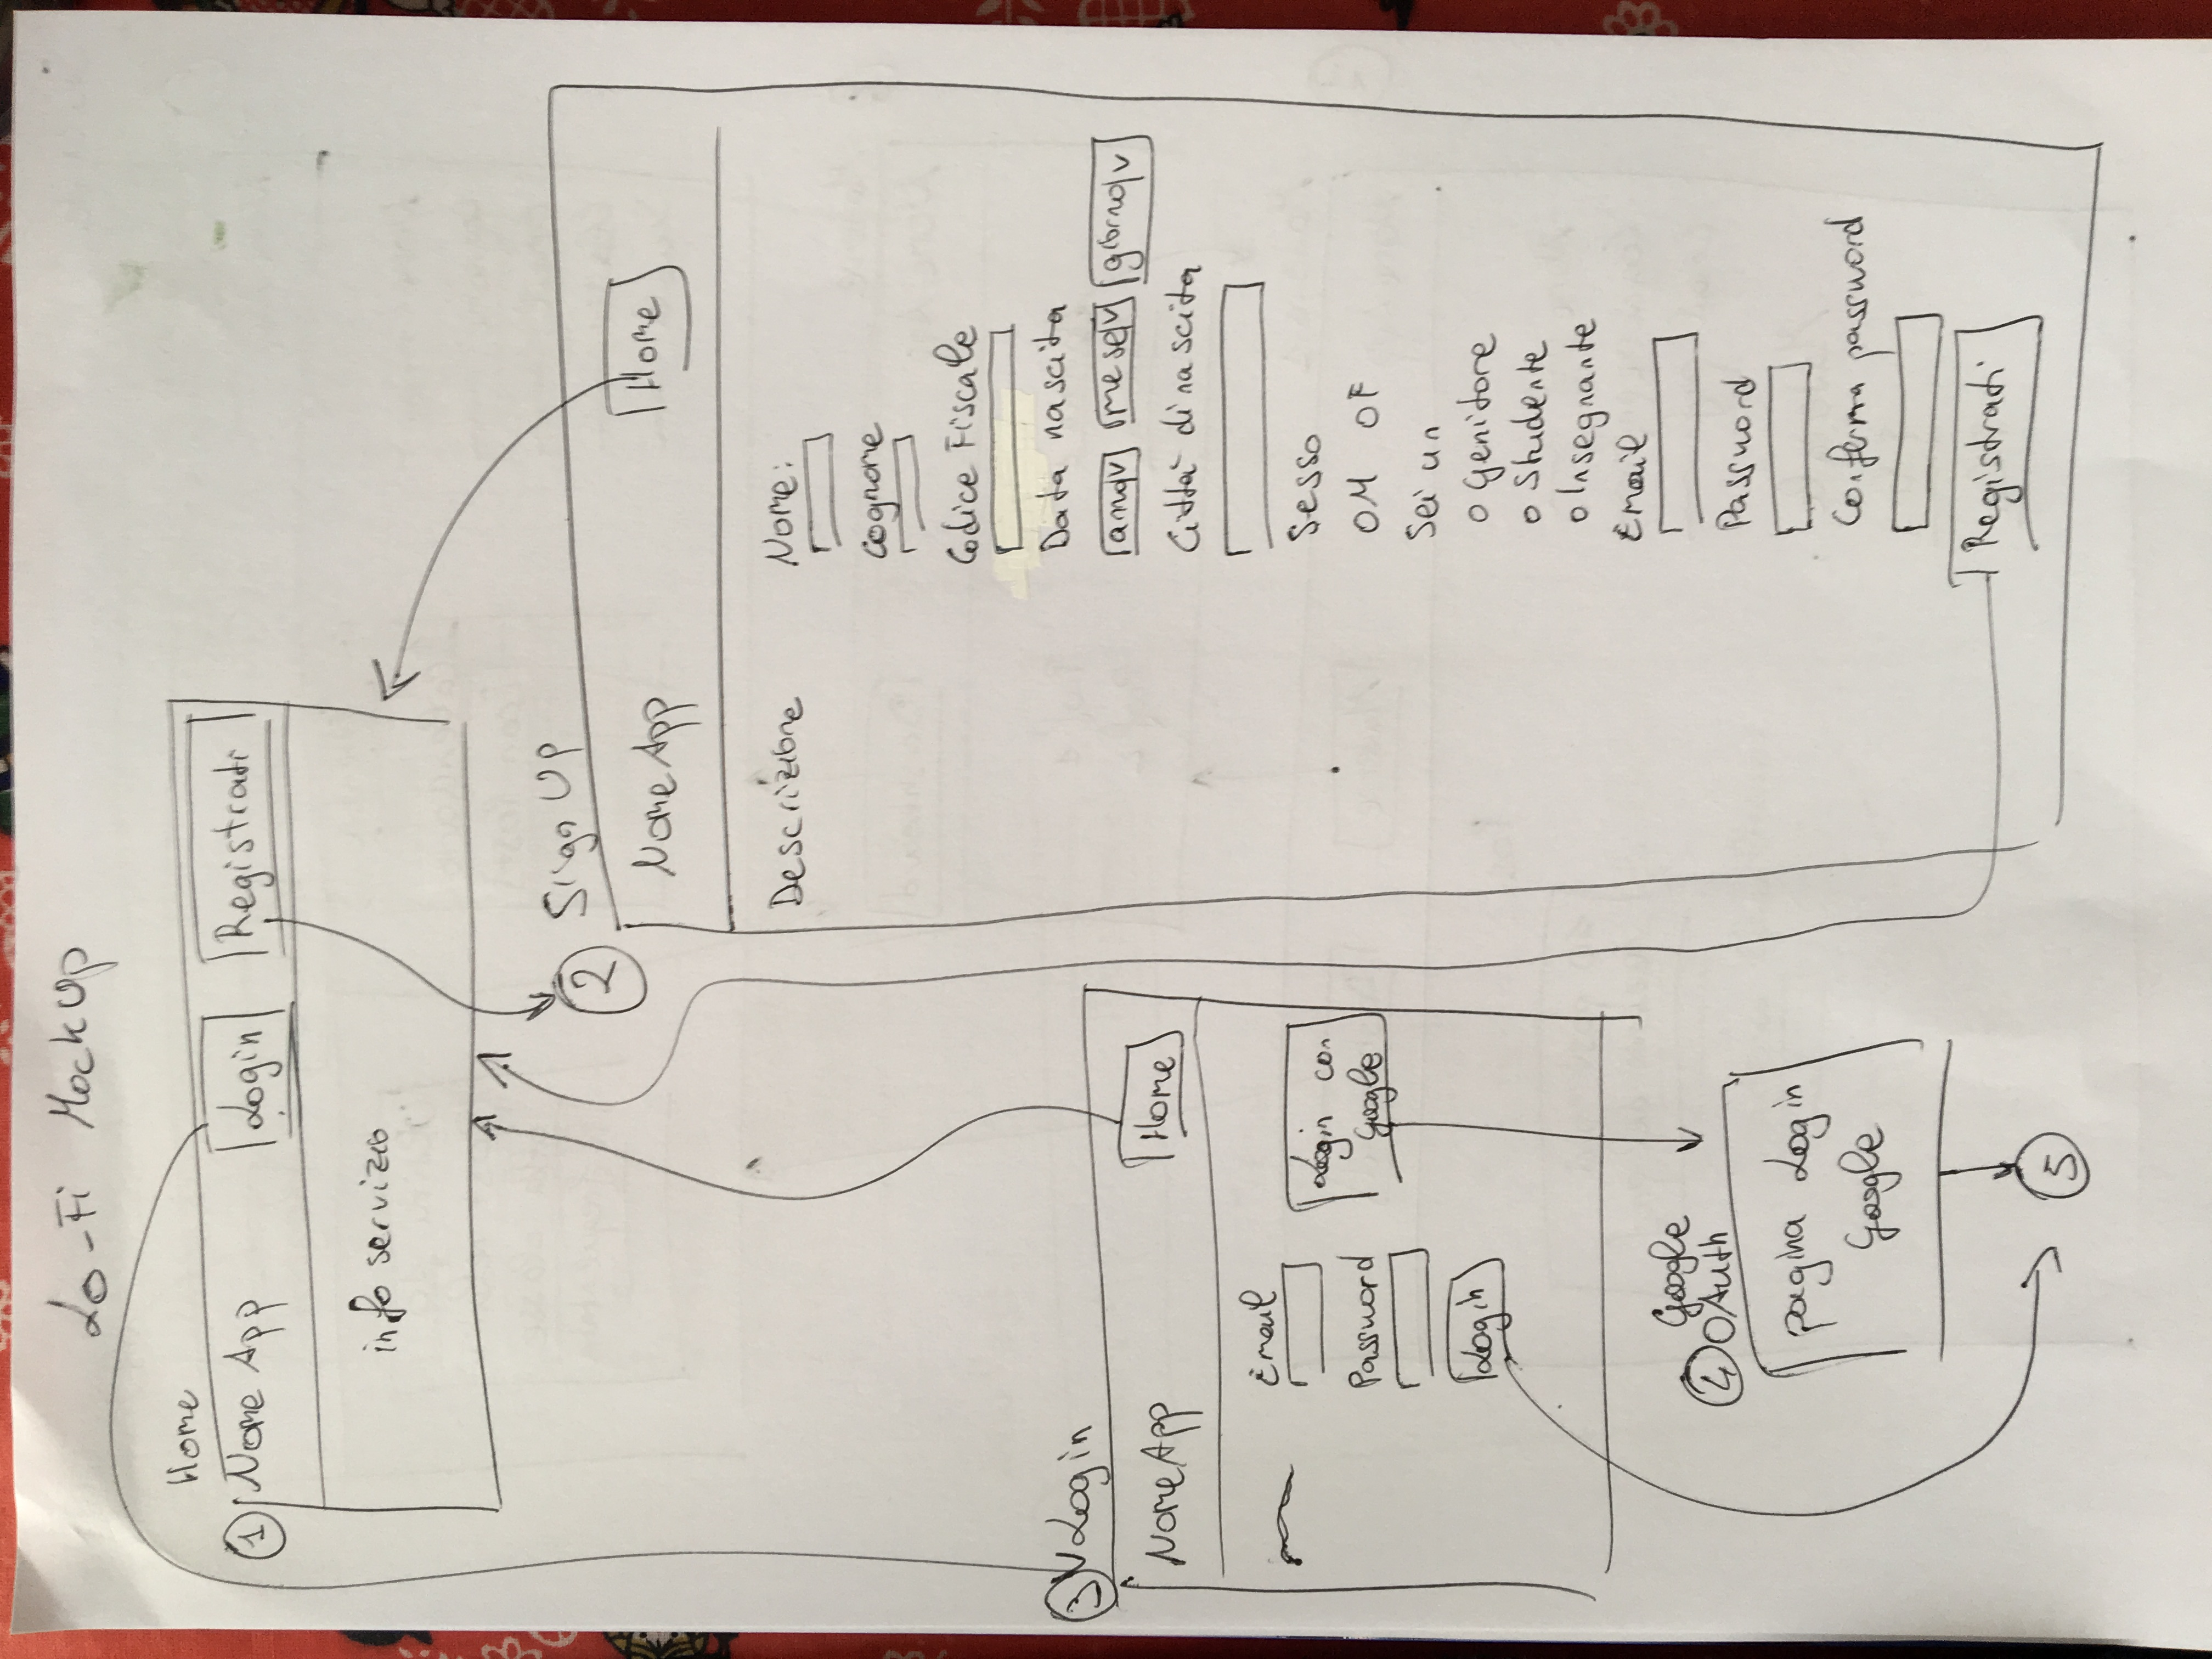
\includegraphics[width=1.3\linewidth, angle=-90]{images/mockup_1}
	\caption{Lo-Fi-Mockup 1}
	\label{fig:mockup_1}
\end{figure}

\begin{figure}[H]
	\centering
	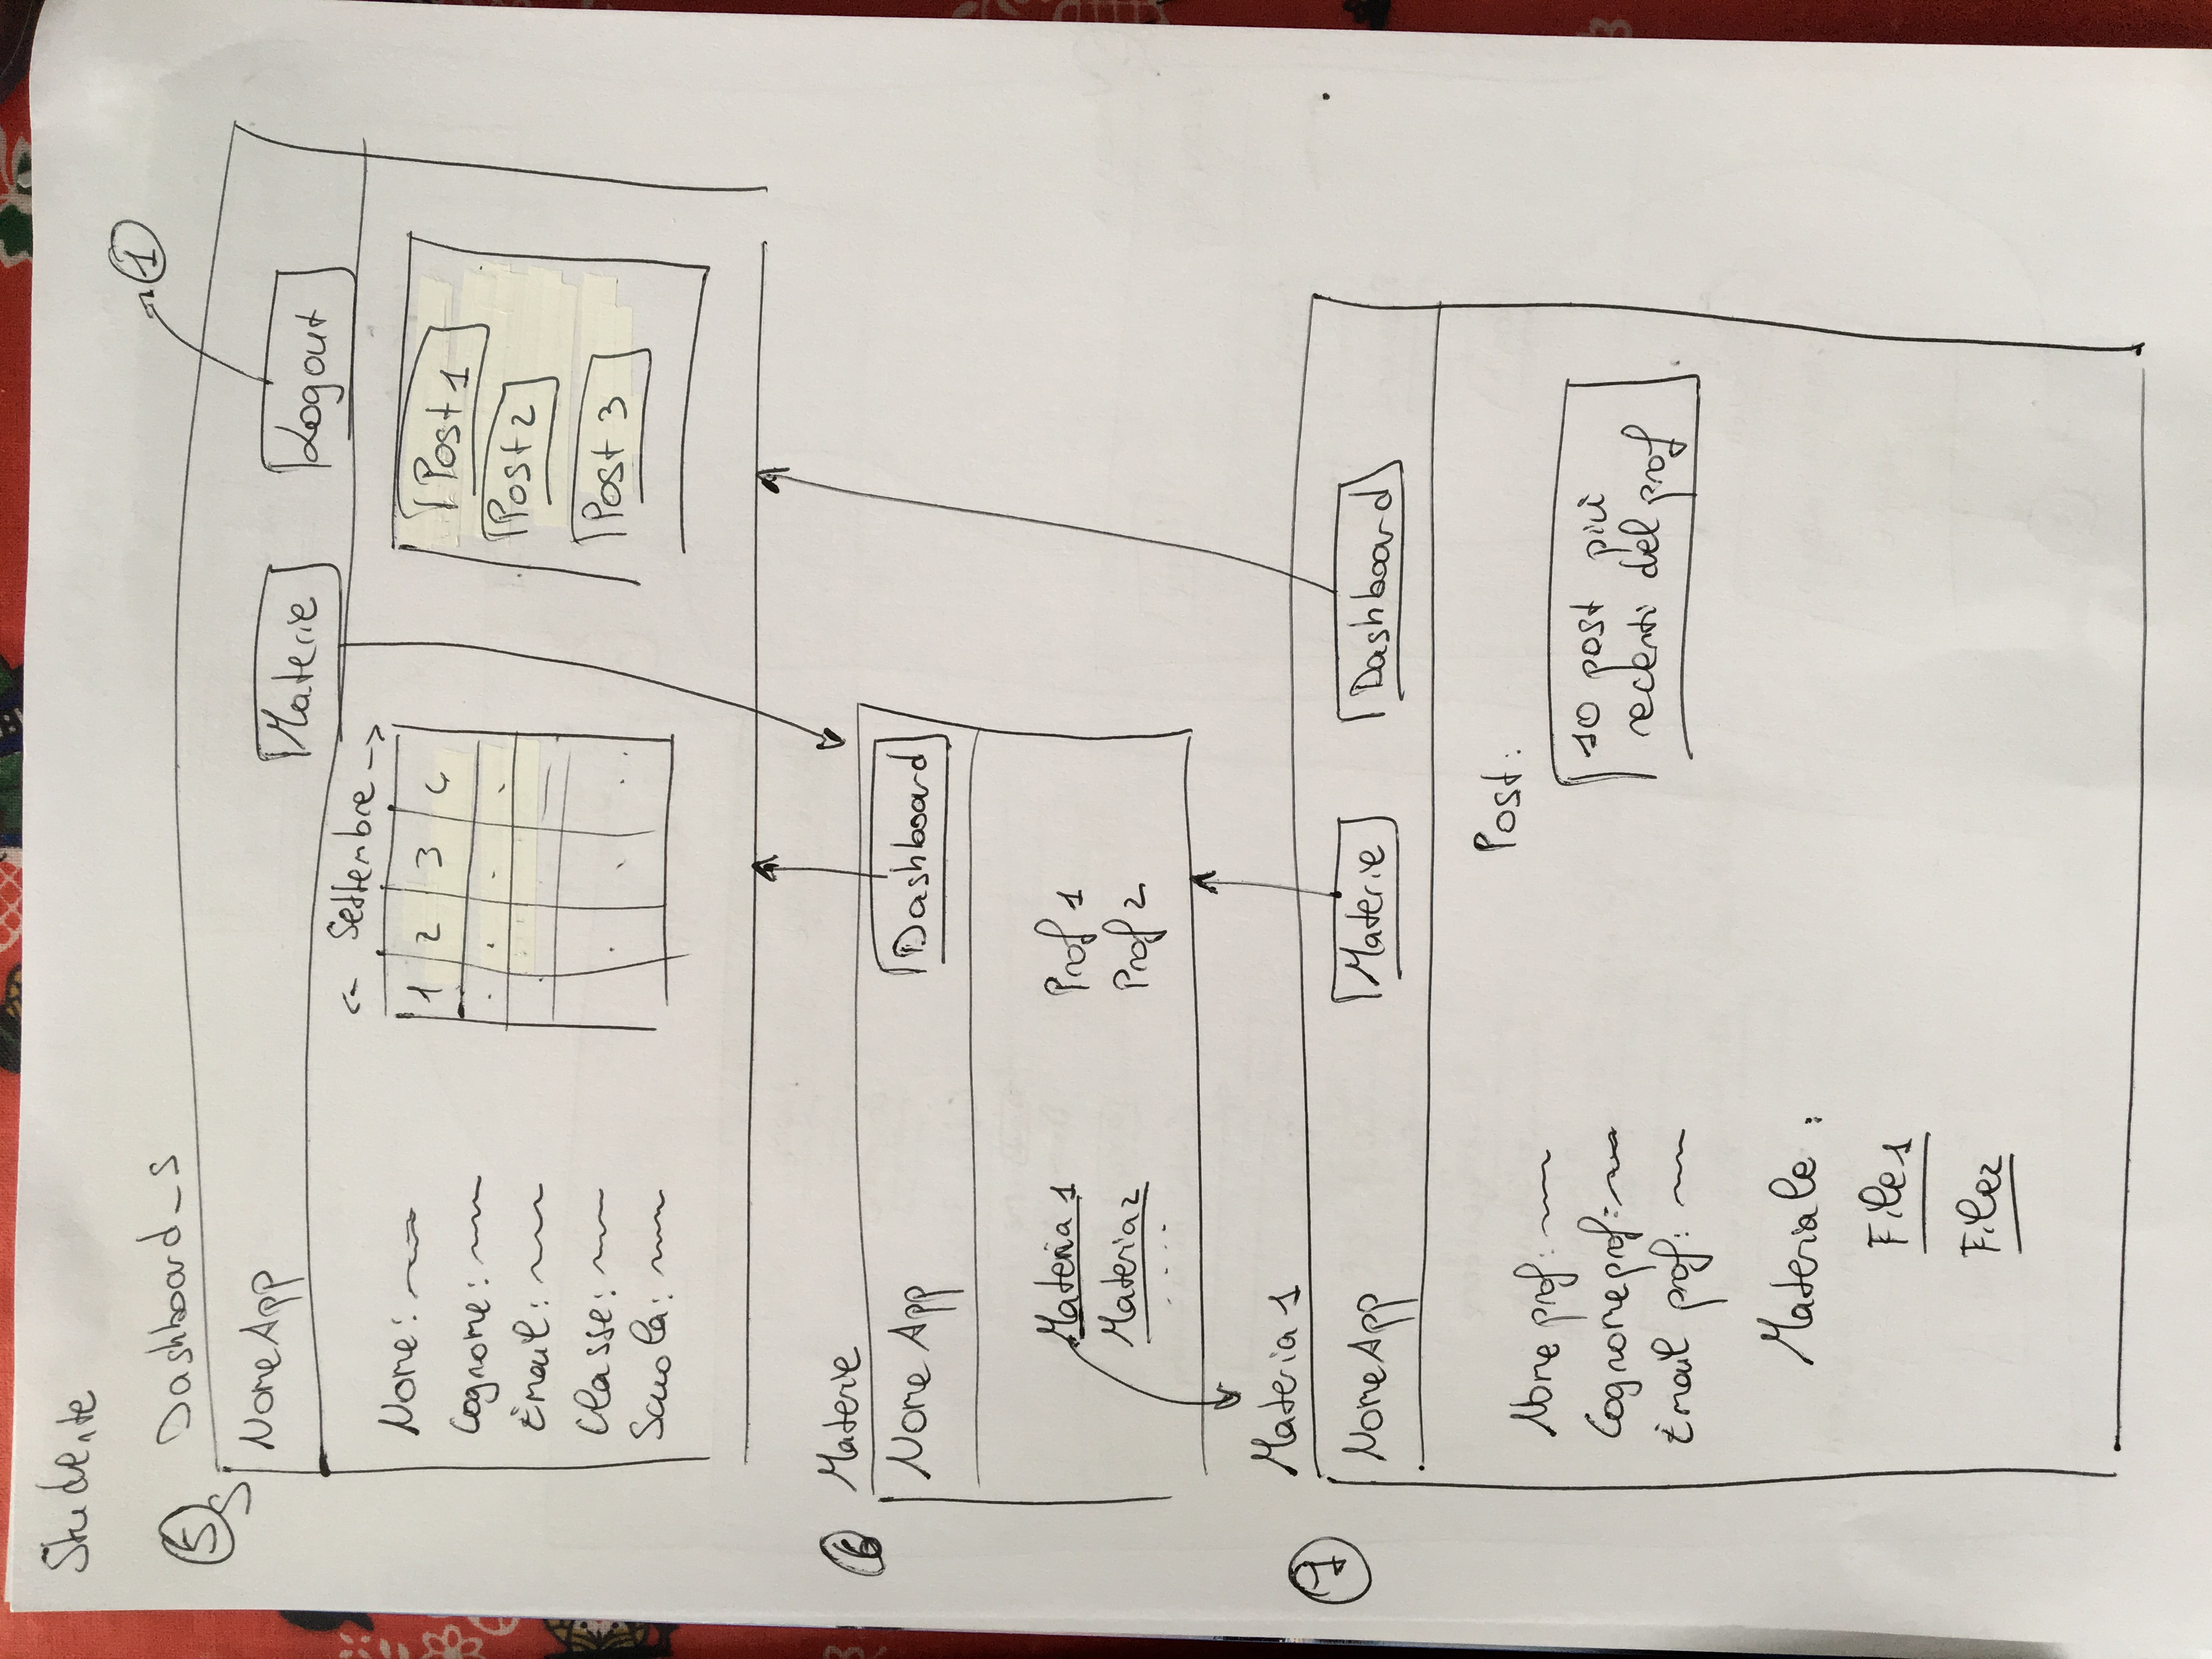
\includegraphics[width=1.3\linewidth, angle=-90]{images/mockup_2}
	\caption{Lo-Fi-Mockup 2}
	\label{fig:mockup_2}
\end{figure}

\begin{figure}[H]
	\centering
	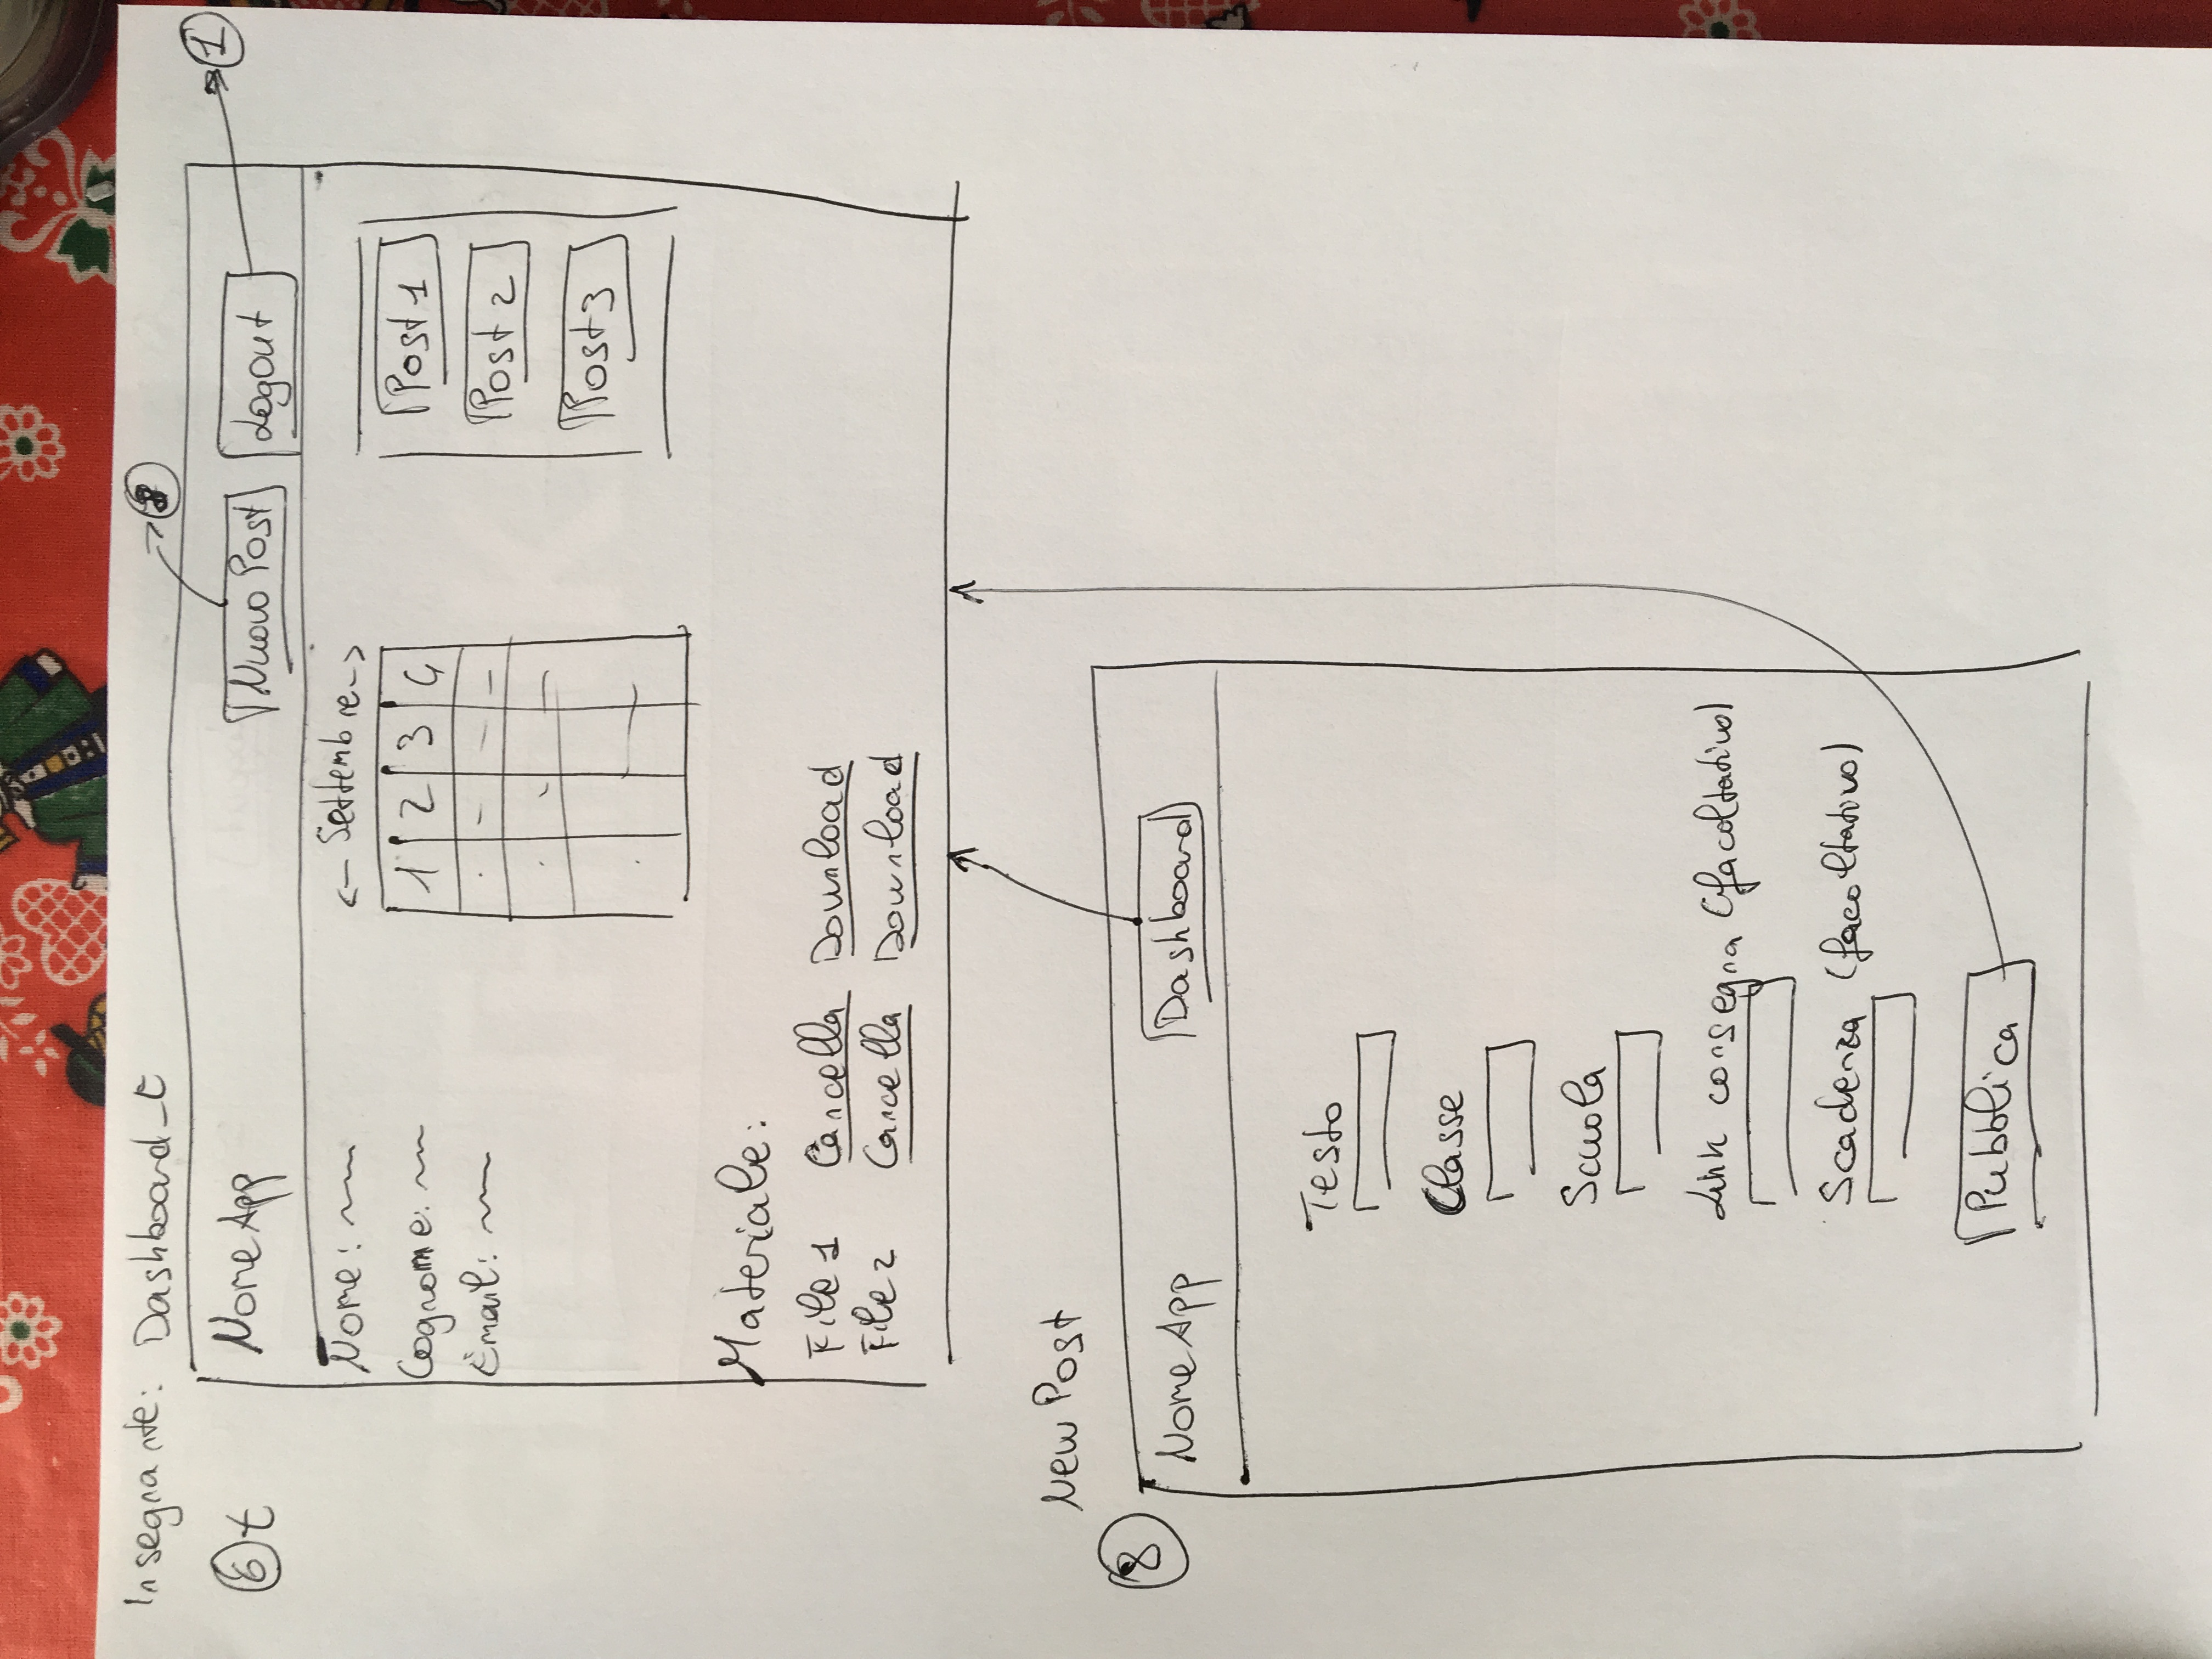
\includegraphics[width=1.3\linewidth, angle=-90]{images/mockup_3}
	\caption{Lo-Fi-Mockup 3}
	\label{fig:mockup_3}
\end{figure}

\begin{figure}[H]
	\centering
	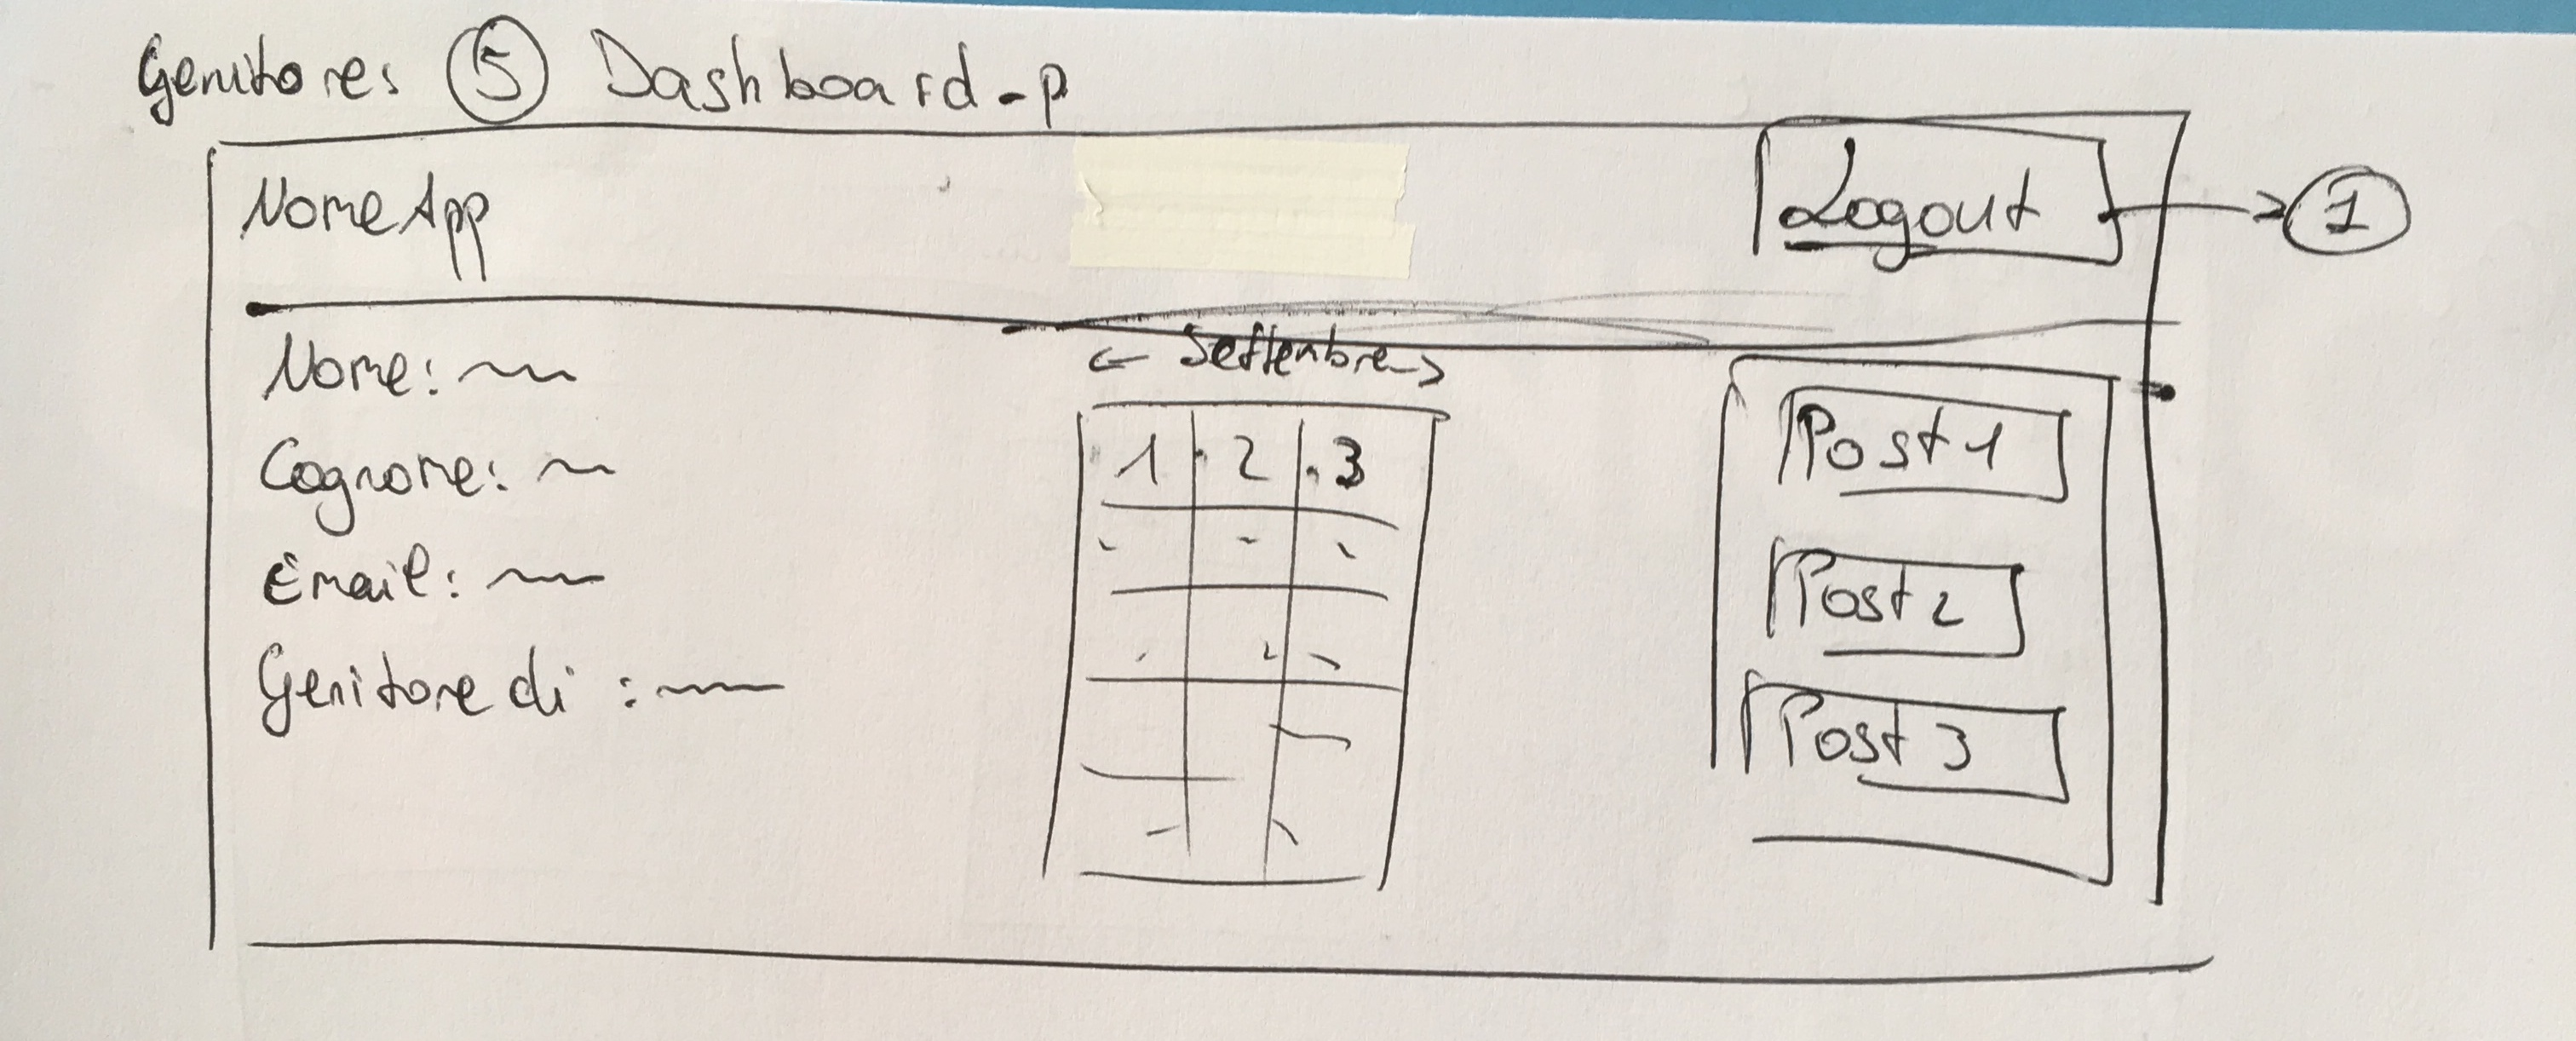
\includegraphics[width=1\linewidth]{images/mockup_4}
	\caption{Lo-Fi-Mockup 4}
	\label{fig:mockup_4}
\end{figure}

\subsection{User Stories}
Di seguito si riporta l'elenco delle user stories: descrivono brevemente ma in maniera efficace le azioni che verranno implementate fornendo i servizi precedentemente descritti agli utenti.\\

\begin{enumerate}
	\item \textbf{Go to the "SignUp" page from the "Home" page}\\
			As a user\\
			So that I can sign up\\
			Given I'm in the "Home" page\\
			When I press the button "SignUp"\\
			Then I should be in the "SignUp" page\\
	\item \textbf{SignUpAs a user}\\
			So that I can use the app's services\\
			Given I'm in the "SignUp" page\\
			When I fill the form correctly\\
			and I press the button "SignUp"\\
			Then I should be registered in the app\\
			and I should be in the "Home" page\\
	\item \textbf{Return to the "Home" page from the "SignUp" page}\\
			As a user\\
			So that I can return to the "Home" page without signing up\\
			Given I’m in the "SignUp" page\\
			When I press the button "Home"\\
			Then I should be in the "Home" page\\
	\item \textbf{Go to the "LogIn" page from the "Home" page}\\
			As a user\\
			So that I can login\\
			Given I’m in the "Home" page\\
			When I press the button "Login"\\
			Then I should be in the "Login" page\\
	\item \textbf{LogIn without Google}\\
			As a user\\
			So that I can use the app’s services\\
			Given I’m in the "LogIn" page\\
			and that I’ve signed up as a "Parent"\\
			When I fill the form correctly\\
			and I press the button "LogIn"\\
			Then I should be logged in as a "Parent"and I should be in the "Dashboard\_g" page\\
	\item \textbf{LogIn with Google}\\
			As a user\\
			So that I can use the app’s services\\
			Given I’ve signed up as a "Student" or as a "Teacher"\\
			I want to log in with Google OAuth\\
	\item \textbf{Go to the "Home" page from the "LogIn" page}\\
			As a user\\
			So that I can return to the "Home" page without logging in\\
			Given I’m in the "LogIn" page\\
			When I press the button "Home"\\
			Then I should be in the "Home" page\\
	\item \textbf{LogOut}\\
			As a user\\
			So that I can stop using the app’s services\\
			Given I’m in the correct "Dashboard\_*" page\\
			When I press the button "LogOut"\\
			Then I should have logged out correctly\\
			and I should be in the "Home" page\\
	\item \textbf{Calendar}\\
			As a user\\
			So that I can know the current date and organize my work properly\\
			Given I’m in the correct "Dashboard\_*" page\\
			Then I should see the current date\\
	\item \textbf{Posts seen by "Student"As a "Student"}\\
			So that I can see the posts all my "Teacher"s made\\
			Given I’m on the "Dashboard\_s" page\\
			Then I should see the 10 most recent posts\\
	\item \textbf{Go to the "Dashboard\_*" page}\\
			As a user\\
			So that I can go to the "Dashboard\_*" whenever I need it\\
			When I press the button "Dashboard"\\
			Then I should be in the correct "Dashboard\_*" page\\
	\item \textbf{Materie}\\
			As a "Student"\\
			So that I can see the subjects teached at school\\
			Given I’m on the "Dashboard\_s" page\\
			When I press the button "Materie"\\
			Then I should be on the "Materie" page\\
	\item \textbf{Subject info}\\
			As a "Student"\\
			So that I can have more information about a subject\\
			Given I’m in the "Materie" page\\
			When I click che link corresponding to subject *\\
			Then I should be in the page "Materia*" corresponding to subject *\\
	\item \textbf{Go to the "Materie" page from "Materia*" page}\\
			As a "Student"\\
			So that I can go to the "Materie" page from the "Materia*" page\\
			Given I’m in the "Materia*" page\\
			When I press the button "Materie"\\
			Then I should be in the "Materie" page\\
	\item \textbf{Resources for a specific subject}\\
			As a "Student"\\
			So that I can use the resources on subject*\\
			Given I’m in the "Materia*" page\\
			and I see the files that are the resources\\
			When I click the link corresponding to a file\\
			Then I should be able to download that file\\
	\item \textbf{"Teacher"’s posts}\\
			As a "Student"\\
			So that I can have a focus on the specific subject*\\
			Given I’m in the "Materia*" page\\
			Then I should see the 5 most recent posts made by the "Teacher" corresponding to that subject\\
	\item \textbf{Posts seen by "Teacher"}\\
			As a "Teacher"\\
			So that I can see understand the workload my "Student"s have\\
			Given I’ in the "Dahsboard\_t" page\\
			Then I should see the 10 most recent posts made by me and the other "Teacher"s who teach my "Student"s\\
	\item \textbf{Remove a file}\\
			As a "Teacher"\\
			So that I can remove files\\
			Given I’m in the "Dashboard\_t" page\\
			When I click on the “Cancella” link corresponding to the file I want to remove\\
			Then the file corresponding to the link I clicked should be removed\\
	\item \textbf{Download a file}\\
			As a "Teacher"\\
			So that I can download files\\
			Given I’m in the "Dashboard\_t" page\\
			When I clicked on the “Download” link corresponding to the file I want to download\\
			Then the file corresponding to the link I clicked should be downloaded\\
	\item \textbf{Upload a file}\\
			As a user\\
			So that I can upload a file\\
			Given I’m in the "CaricoFile" page\\
			And that I’ve specified what file I want to upload\\
			When I press the button "Aggiungi"\\
			Then the file should be uploaded correctly\\
	\item \textbf{Go to the "NewPost" page from the "Dashboard\_t" page}\\
			As a "Teacher"\\
			So that I can communticate with my "Student"s and assign homework to them\\
			Given I’m in the "Dashboard\_t" page\\
			When I press the button "Nuovo Post"\\
			Then I should be in the "NewPost" page\\
	\item \textbf{Publish a post}\\
			As a "Teacher"\\
			So that I can communicate with my "Student"s and assign homework to them\\
			Given I’m in the "NewPost" page\\
			and that I filled the form correctly\\
			When I press the button "Pubblica"\\
			Then a new post should be published correctly\\
	\item \textbf{Posts seen by a "Parent"}\\
			As a "Parent"\\
			So that I can be updated on my son’s scholastic situationGiven I’m in the "Dashboard\_p" page\\
			Then I should see the posts made by my son’s "Teacher"s\\
\end{enumerate}

\chapter{Tecnologie e Metodologie utilizzate}

\section{Rails e il paradigma Model-View-Controller}

L’applicazione è stata realizzata con Ruby on Rails, seguendo i principi su cui esso è basato, e varie gemme in esso contenuto.\\
In particolare, Rails è un framework per lo sviluppo di applicazioni web SaaS (Software as a Service) scritto in Ruby. Esso è stato sviluppato tenendo a mente le più importanti linee guida nella progettazione e programmazione di questo tipo di software, in particolare i principi fondamentali sono due: Don’t Repeat Yourself (non ci deve essere codice ridondante, ma una singola scrittura efficace delle varie funzionalità e caratteristiche) e Conventions Over Configuratons (bisogna specificare delle configurazioni solo nel caso in cui non si seguano quelle raccomandate naturalmente dal framework).
Tutto ciò è implementato col paradigma Model-View-Controller: i modelli servono per interagire con i dati del sistema, le view li visualizzano in maniera appropriata rendendo possibile l’interazione con gli utenti, mentre i controller ricevono i comandi di questi (solitamente attraverso le view e il browser) e li eseguono.

\subsection{Autenticazione locale}

Per l’autenticazione è stata utilizzata la gemma Canard per implementare un modello di Role-Based Authentication (ulteriori dettagli nella sezione TODO) insieme alla gemma Devise.
Devise è uno strumento molto utile per ogni svilippatore Rails: è organizzata in moduli, per cui è possibile costruire dal più semplice meccanismo di identificazione e verfica, a quello più complesso con diversi servizi aggiuntivi. In questa applicazione sono stati usati soprattutto i seguenti moduli:

\begin{itemize}
	\item \textbf{Database Authenticatable}: memorizza in maniera sicura e cifrata (grazie al supporto della gemma Bcrypt) la password dell’utente nel databse del sistema
	\item \textbf{Registarable}: permette agli utenti di registrarsi
	\item \textbf{Rememberabe}: gestisce le sessioni degli utenti tramite i cookie
	\item \textbf{Validatable}: convalida le email e le password
	\item \textbf{Omniauthable}: gestisce autenticazione tramite OAuth (ulteriori dettagli nella sezione successiva).
\end{itemize}

Ulteriori comodità di questa gemma sono le route e le view da essa create automaticamente per tutti i processi relativi all’autenticazione, personalizzabili in maniera opportuna

\subsection{Autenticazione tramite Google OAuth}

OAuth è un protocollo di rete basato su HTTP che consente di delegare l’autenticazione ad una terza entità (quale potrebbe essere Google, Facebook, Twitter...). In esso sono definiti quattro ruoli principali:

\begin{enumerate}
	\item \textbf{Utente} (Resource Owner): è il possessore dell’account, e deve autorizzare l’accesso alle informazioni contenute in esso e alle risorse protette conservate nel Resource Server
	\item \textbf{Client} (Consumer): è l’applicazione che vorrebbe accedere alle informazioni e risorse dell’Utente, di cui chiede l’autorizzazione
	\item \textbf{Resource Server}: il server dove si trovano le risorse protette dell’Utente
	\item \textbf{Authorization Server}: è il server che si occupa di richiedere all’Utente di autenticarsi (con le credenziali di quest’ultimo) per autorizzare l’accesso alle sue risorse
\end{enumerate}

Lo schema di funzionamento è descritto dalla seguente immagine:\\

\begin{figure}[H]
	\centering
	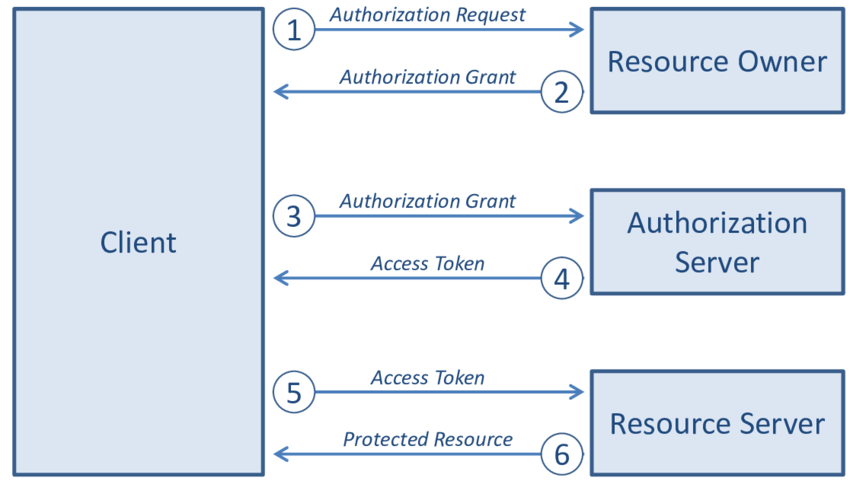
\includegraphics[width=0.90\linewidth]{images/oauth}
	\caption{OAuth Flow}
	\label{fig:oauth}
\end{figure}

In questo caso, l’Authorization Server e il Resource Server coincidono (Google), mentre il ruolo del client è svolto dalla nostra applicazione.\\
Per implementare tutto ciò ci si è serviti, come accennato in precedenza, del modulo Omniauthable di Devise in aggiunta alla gemma \textit{omniauth-googleoauth2}.

\subsection{Google Drive}

Come affermato in precedenza, per memorizzare le risorse a disposizione degli studenti si è usato Google Drive.\\
La prima cosa da fare è stato associare all'applicazione un service account dalla Google API Console. Un service account è un particolare account Google che rappresenta un' entità non umana che necessita di accedere a delle risorse protette. Di conseguenza all'applicazione in esame sono stati associate una email, una password e un ID per Google.\\
Per gestire i file (upload, download) ed intergire con questo servizio è stata usata la gemma \textit{google-api-client}.

\subsection{Altre gemme}

Per una più completa trattazione dello sviluppo si è cominciato ad impostare il deploy su Heroku, tramite le gemme \textit{rails\_12factor}(perconfigurare l'ambiente di produzione dell'applicazione), \textit{pg} (in quanto il database di Heroku è basato su PostgreSQL e non SQLite usato per lo sviluppo) e \textit{figaro} (per gestire le chiavi e gli ID segreti negli ambienti di sviluppo e produzione).\\
Per realizzare il calendario nella Dashboard degli utenti si è usata \textit{simple\_calendar}.\\
Di seguito è riportato il \textit{Gemfile} con tutte le gemme utilizzate:\\


\lstinputlisting[style=Ruby, caption=Gemfile, label=lst:gemfile]{code/Gemfile}
Una discussione degli strumenti usati per i test si può trovare nella sezione TODO\\

\section{Agile per lo sviluppo software}

Nel realizzare questa applicazione mi sono ispirata alla metodologia Agile. Essa è in realtà pensata per gruppi di persone che lavorano insieme allo stesso software: le interazione tra i vari membri di un singolo team e tra i responsabili di questi hanno un'enorme importanza, e sono il vero punto di forza di questa metodologia, insieme al contatto con il committente.\\
Nonostante ciò, in questo lavoro ho voluto tenere fede ai principi di Behavior-Driven Design e Test-Driven Development. Di conseguenza, prima dello sviluppo del codice, nella fase di progettazine, sono stati realizzati i lo-fi mockup e le user stories per fare chiarezza su cosa doveva essere realizzato. Successivamente, durante lo sviluppo, per ogni user story veniva scritto un test e il codice per soddisfarlo, in modo che tutto fosse fatto in modo corretto. Ponendo l'attenzione sulla qualità e sui contenuti da subito si sono evitati lunghi e tortuosi processi di debug, oltre all'implementazione di funzionalità inutili o non richieste.

\subsection{Tool per applicare al meglio Agile}

Per applicare al meglio la metologia Agile e lavorare efficientemente ho utilizzato i seguenti strumenti:

\begin{itemize}
	\item \textbf{Git}: per il versioning control. La repository su cui è conservato il progetto è la seguente: \url{https://github.com/SilviadelPiano/HiSchool.git}
	\item \textbf{Visual Studio Code} come editor
	\item \textbf{Draw.io} per la reailzzazione degli schemi ER e UML
	\item \textbf{Pivotal Tracker} per il tracking degli sprint e per monitorare i progressi e l'andamento del lavoro. Il link alla pagina corrispondente all'applicazione in esame è il seguente: \url{https://www.pivotaltracker.com/n/projects/2393952}
\end{itemize}

\chapter{Analisi Concettuale del Sistema}

\section{Schema Entità-Relazione}
In questa sezione viene riportato lo schema ER del databse. Come si può vedere esso rappresenta i requisiti descritti nella sezione \ref{requisiti_db}, assieme ad altri vincoli necessari per lo sviluppo di questa applicazione.
Sono indicati anche gli identificatori principali.

\begin{figure}[H]
	\centering
	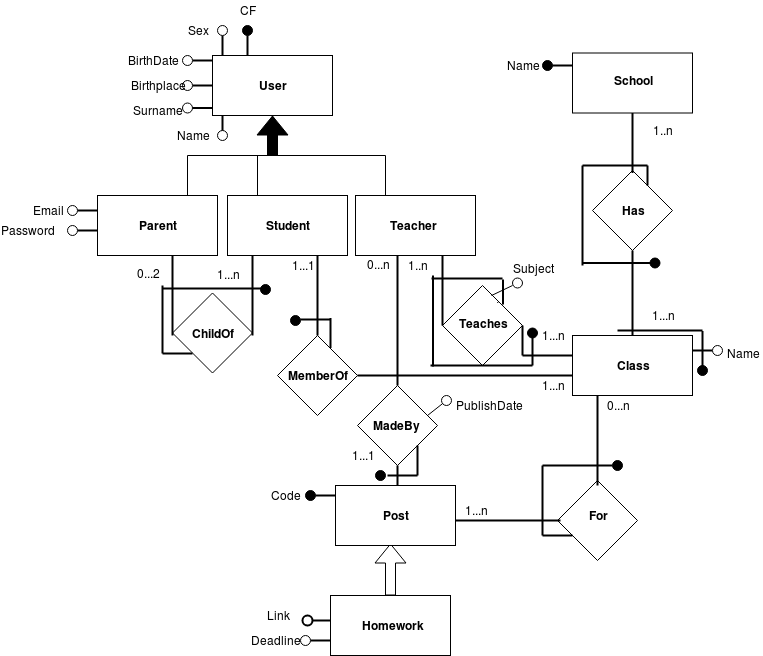
\includegraphics[width=1\linewidth]{images/db_HiSchool.png} 
	\caption{Schema ER}
	\label{fig:schema_ER}
\end{figure}

\section{Elenco delle entità e delle relazioni}

In questa sezione verranno presentate in maniera più approfondita le varie entità e relazioni situate nello schema.
\subsection{Generalizzazione User}
\textbf{User} è l'entità che rappresenta l'utente che andrà ad usufruire dell'applicazione: si può notare infatti la generalizzazione che differenzia i tre tipi di utilizzatori che si avranno.\\
\textbf{Parent} e \textbf{Student}, cioè le entità che rappresentano il genitore e lo studente, sono legate dalla relazione \textbf{ChildOf}: essa esprime la parentela tra lo studente iscritto e il genitore (potrebbe essere anche il tutore legale del ragazzo in mancanza di parenti più stretti) dello stesso. Un Parent per registrarsi sulla piattaforma deve avere almeno un figlio Student registrato su di essa. D'altro canto, uno Student non deve per forza avere un Parent ad esso associato per registrarsi, ma può averne al massimo 2 associati ad esso.\\
Durante la ristrutturazione Parent, Student e Teacher sono state accorpate a User per generare un'unica entità omonima, dove i vari ruoli sono distinti da un flag, tramite l'ausilio della gemma Canard.

\subsection{Entità School e Class}
L'entità \textbf{School} rappresenta la scuola registrata nel database dell'applicazione, ed è legata a \textbf{Class} tramite la relazione \textbf{Has}. Class è infatti identificata dal proprio nome e dalla Scuola a cui appartiene. Per esempio, la classe 1\ap{a} del liceo scientifico sarà presente in tutti i licei scientifici, ed almeno in 1, altrimenti non esisterebbe, da qui l'associazione 1...n. Una Scuola deve avere almeno una classe.\\
La relazione \textbf{Teaches} esprime l'incarico di insegnamento conferito ad un \textbf{Teacher} (insegnante) nei confronti della classe, ed è presente anche la materia (subject) oggetto di lezione. Ogni classe può essere presa in carico da diversi insegnanti, ma ne deve avere almeno 1 (si pensi solo alle varie materie presenti in  un liceo) ed un singolo insegnante, per essere tale, deve fare lezione ad almeno un classe, ma può averne affidate più di una.\\
La relazione \textbf{MemberOf} invece esprime il fatto che ogni classe debba essere frequentata da almeno uno studente, e questo per essere tale deve, e può, essere iscritto ad una sola classe.\\
Nella ristruttrazione Class e Has sono state accorpate per generare un'unica entità che tenga traccia del nome della classe e della scuola ad essa associata. School rimane singolarmente, in modo che nel futuro sia possibile associare ad essa più classi. Inoltre, al momento della registrazione
all'utente viene chiesto di specificare una classe ed una scuola (in diversi punti dei form da compilare a seconda del ruolo), e sono effettuati due controlli: si verifica l'esistenza della singola scuola (School) nel database, e poi si verfica che per questa sia registrata la classe dichiarata nel form tramite l'entità appena creata con l'accorpamento. Quest'ultima è utile anche per motivi di efficienza del codice.

\subsection{Entità Post}
L'entità \textbf{Post} rappresenta le comunicazioni che possono essere fatte sulla piattaforma. Ogni Post deve essere creato da un singolo insegnante secondo quanto espresso dalla relazione \textbf{MadeBy}, mentre un insegnante non ha l'obbligo di creare Post, e non c'è limite a quanti ne può fare. L'attributo PublishDate registra la data della pubblicazione.
Da notare gli attributi facoltativi Link e Deadline. Essi sono stati inseriti per fornire maggiori opzioni al fine di rendere più efficaci le comunicazioni: come insegnante vorrei poter mettere in evidenza un link dove trovare materiale utile oppure una scadenza o una data importante relativa alla comunicazione appena publicata (che sarà segnata sul calendario).\\
Un Post deve essere associato ad almeno una classe, secondo quanto indicato dalla relazione \textbf{For}, in modo che i suoi membri possano vederlo.

\chapter{Progettazione del sistema (fallo per ultimo, vedi se riesci coi tempi. Vedi quello che ha fatto Jessica}

\section{Archittura del sistema}

\subsection{Architettura dei Controller}

Schema UML da fare con Draw.io dei controller. Vanno inseriti tutti i metodi

\subsection{Architettura delle View}

Schema UML da fare con Draw.io delle view. 

\subsection{Architettura dei Model}

Schema UML da fare con Draw.io dei model 

\section{Progettazione logica del Data Layer}

Breve introduzione di come Rails gestisce il database (prendila dalla guida su Internet)

Nel rispetto dei vincoli relazionali sopra espressi e tenendo conto delle caratteristiche di Rails, lo schema del database è definito nel file \textit{db/schema.rb} modificato, come espresso in precedenza, dai file contenuti nella cartella \textit{db/migrate/}.

\lstinputlisting[style=Ruby, caption=db/schema.rb, label=lst:dbschema]{code/schema.rb}



\end{document}